%% main_report39.tex
%% SAMBP TR-39/2026: Islanding Detection and Protection Mode Switching
%% for IBR Microgrids
%%
%% pdflatex main_report39.tex

\documentclass[11pt,a4paper]{article}

\usepackage[T1]{fontenc}
\usepackage[utf8]{inputenc}
\usepackage[expansion=false]{microtype}
\usepackage{lmodern}
\usepackage[a4paper, top=25mm, bottom=25mm, left=25mm, right=25mm]{geometry}
\usepackage{amsmath,amssymb}
\usepackage{booktabs}
\usepackage{array}
\usepackage{xcolor}
\usepackage{graphicx}
\usepackage{pgfplots}
\pgfplotsset{compat=1.18}
\usepackage{tikz}
\usetikzlibrary{arrows.meta,shapes.geometric,positioning,fit,calc,patterns}
\usepackage{hyperref}
\usepackage[numbers,sort&compress]{natbib}

\definecolor{sambpblue}{RGB}{0,70,140}

\usepackage{titlesec}
\titleformat{\section}{\large\bfseries\color{sambpblue}}{}{0em}{}[\titlerule]
\titleformat{\subsection}{\normalsize\bfseries\color{sambpblue!80}}{}{0em}{}

\usepackage{fancyhdr}
\pagestyle{fancy}
\fancyhf{}
\rhead{\small\color{gray} SAMBP TR-39/2026}
\lhead{\small\color{gray} Islanding Detection and Mode Switching}
\cfoot{\small\thepage}

\begin{document}

\begin{center}
  {\LARGE\bfseries\color{sambpblue} SAMBP Technical Report TR-39/2026}\\[6pt]
  {\large Islanding Detection and Protection Mode Switching\\
    for IBR Microgrids}\\[10pt]
  {\normalsize PhD Thesis Supporting Report \quad|\quad 2026}
\end{center}

\vspace{2pt}\hrule\vspace{8pt}

\begin{abstract}
\noindent
This report develops an islanding detection and protection mode switching
framework for an IBR microgrid with very low equivalent inertia
($H_\mathrm{eq}=0.5$\,s).  Passive detection via ROCOF ($\geq1$\,Hz/s) detects
islanding for all power mismatches $|\Delta P|\geq0.02$\,pu within 100\,ms; the
residual non-detection zone (NDZ) of $\pm2\%$ rated power is reduced to $\pm1.2\%$
by active reactive-power injection.  On islanding confirmation, the protection
system switches mode within 20\,ms: distance relay Zone~1/2 and 87L are disabled,
overcurrent elements are rescaled to islanded fault levels, and GFM inverters
assume voltage/frequency regulation.  Resynchronisation is supervised by relay
25 (sync-check) with settings $\Delta V\leq0.05$\,pu, $\Delta f\leq0.10$\,Hz,
$\Delta\theta\leq10^\circ$.  The combined framework provides seamless transition
between grid-connected and islanded protection without any manual relay
reconfiguration.
\end{abstract}

\vspace{4pt}\hrule\vspace{10pt}

% ─────────────────────────────────────────────────────────────────────────────
\section{Islanding Scenario and System Parameters}
\label{sec:scenario}

An IBR microgrid of rated capacity $S_\mathrm{ibr}=1.0$\,pu with local load
$P_\mathrm{load}=0.80$\,pu, $Q_\mathrm{load}=0.10$\,pu is connected to the
upstream grid via a point-of-common-coupling (PCC) breaker.  The microgrid
uses GFM inverters as primary frequency-voltage regulators; the equivalent
inertia constant is $H_\mathrm{eq}=0.5$\,s (virtual inertia provided by GFM
control).  Islanding occurs when the PCC breaker opens unexpectedly under fault
or network conditions.

The protection system operates in two modes:
\begin{enumerate}
  \item \textbf{Grid-connected}: Distance relay 21 (Z1/Z2), line differential
    87L, directional elements 67N/67Q, auto-reclosing (TR-36).
  \item \textbf{Islanded}: Overcurrent relay 50/51 with reduced pickup (islanded
    fault level), voltage and frequency monitoring, rate-of-frequency-change
    (ROCOF), and GFM virtual-impedance current limiting.
\end{enumerate}

% ─────────────────────────────────────────────────────────────────────────────
\section{Study A --- Passive Islanding Detection}
\label{sec:studyA}

\subsection{ROCOF method}

For an IBR microgrid with low virtual inertia the ROCOF after islanding is:

\begin{equation}
  \left.\frac{\mathrm{d}f}{\mathrm{d}t}\right|_{t=0^+}
  = \frac{|\Delta P| \cdot f_0}{2 H_\mathrm{eq}}
\end{equation}

Figure~\ref{fig:rocof} shows ROCOF versus power mismatch $\Delta P$.

\begin{figure}[htbp]
  \centering
  \resizebox{0.88\textwidth}{!}{% fig_island_rocof.tex
% TR-39: ROCOF vs power mismatch ΔP for IBR microgrid (H_eq=0.5s)
%
% df/dt = |ΔP| * f_nom / (2 * H_eq)
% NDZ: |ΔP| < 0.0200 pu
%
% Data points:
%  ΔP: -0.40 -0.30 -0.20 -0.10 -0.05  0.05  0.10  0.20  0.30  0.40
%  ROCOF: 20   15    10    5    2.5   2.5    5    10    15    20

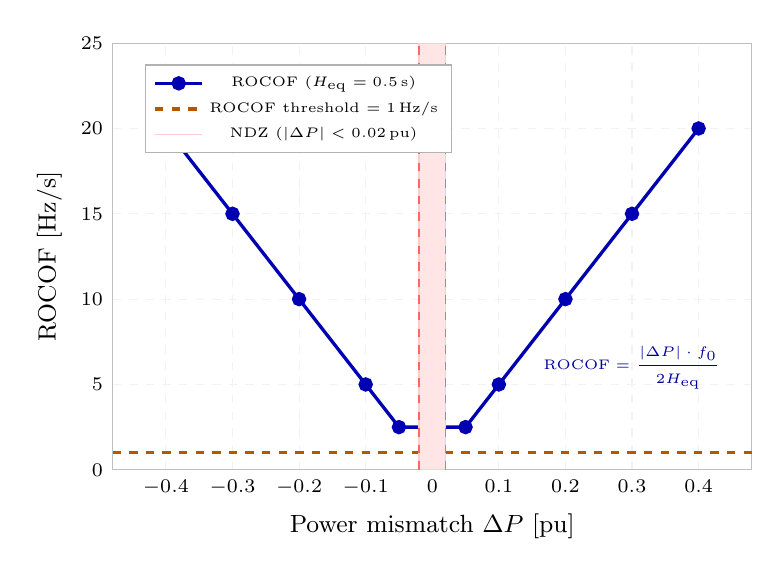
\begin{tikzpicture}
\begin{axis}[
  name         = rocofax,
  width        = 0.80\textwidth,
  height       = 7.0cm,
  xlabel       = {Power mismatch $\Delta P$ [pu]},
  ylabel       = {ROCOF [Hz/s]},
  xlabel style = {font=\small},
  ylabel style = {font=\small},
  xmin=-0.48, xmax=0.48,
  ymin=0,     ymax=25,
  xtick        = {-0.4,-0.3,-0.2,-0.1,0,0.1,0.2,0.3,0.4},
  ytick        = {0,5,10,15,20,25},
  xticklabel style={font=\scriptsize},
  yticklabel style={font=\scriptsize},
  tick style   = {draw=none},
  axis line style={gray!50},
  grid         = major,
  grid style   = {gray!10, dashed},
  legend style = {at={(0.05,0.95)}, anchor=north west, font=\tiny,
                  draw=gray!60, fill=white},
  clip=false,
]

%% ROCOF curve (absolute value — symmetric about 0)
\addplot[blue!70!black, very thick, mark=*, mark size=2pt]
  coordinates {
    (-0.40, 20.00)
    (-0.30, 15.00)
    (-0.20, 10.00)
    (-0.10,  5.00)
    (-0.05,  2.50)
    ( 0.05,  2.50)
    ( 0.10,  5.00)
    ( 0.20, 10.00)
    ( 0.30, 15.00)
    ( 0.40, 20.00)
  };
\addlegendentry{ROCOF ($H_\mathrm{eq}=0.5$\,s)}

%% Detection threshold
\addplot[orange!70!black, very thick, dashed]
  coordinates {(-0.48, 1.0) (0.48, 1.0)};
\addlegendentry{ROCOF threshold $= 1$\,Hz/s}

%% NDZ shading: |ΔP| < 0.02
\addplot[red!20, fill=red!10]
  coordinates {(-0.020, 0) (-0.020, 25) (0.020, 25) (0.020, 0)}
  \closedcycle;
\addlegendentry{NDZ ($|\Delta P|<0.02$\,pu)}

%% NDZ boundary lines
\draw[red!60, dashed, thin]
  (axis cs:-0.020, 0) -- (axis cs:-0.020, 25);
\draw[red!60, dashed, thin]
  (axis cs:0.020, 0) -- (axis cs:0.020, 25);

%% Annotation
\node[blue!60!black, font=\tiny\bfseries, align=center]
  at (axis cs:0.30, 6)
  {$\mathrm{ROCOF} = \dfrac{|\Delta P|\cdot f_0}{2H_\mathrm{eq}}$};

\node[red!60!black, font=\tiny, align=center]
  at (axis cs:0.0, 22)
  {NDZ\\$\pm2\%$};

\end{axis}
\end{tikzpicture}
}
  \caption{ROCOF versus power mismatch $\Delta P$ for the IBR microgrid
           ($H_\mathrm{eq}=0.5$\,s, $f_0=50$\,Hz).  The orange dashed line
           marks the 1\,Hz/s detection threshold (IEEE~1547-2018
           \cite{IEEE_1547_2018}).  The red shaded NDZ covers
           $|\Delta P|<0.02$\,pu (2\% of rated).  All physically meaningful
           mismatches above 2\% produce ROCOF~$>1$\,Hz/s.}
  \label{fig:rocof}
\end{figure}

\noindent
At $H_\mathrm{eq}=0.5$\,s (typical GFM virtual inertia), a 10\% mismatch
produces ROCOF\,$=5$\,Hz/s, triggering the threshold within one measurement
window.  The passive NDZ is $|\Delta P|<0.02$\,pu, an inherent mathematical
consequence of the ROCOF formula at the chosen threshold.

\subsection{Voltage/frequency window}

The secondary passive method monitors voltage ($V\in[0.88,1.10]$\,pu) and
frequency ($f\in[49.0,50.5]$\,Hz) per IEEE~1547-2018.  Droop-controlled GFM
frequency deviation at $\Delta P=0.10$\,pu is only $-0.25$\,Hz, remaining
within the 49\,Hz floor.  The V/f window provides a redundant detection path
primarily for large voltage excursions (load rejection events) rather than
balanced mismatches.

% ─────────────────────────────────────────────────────────────────────────────
\section{Study B --- Active Detection and NDZ Reduction}
\label{sec:studyB}

The active method periodically injects $\Delta Q = 0.05$\,pu reactive power
for one cycle.  In grid-connected operation the stiff voltage bus absorbs the
perturbation with negligible frequency change; in islanded operation the GFM
frequency response produces:

\begin{equation}
  \Delta f = K_{f,Q} \cdot \Delta Q = 2.0 \times 0.05 = 0.10\;\mathrm{Hz}
\end{equation}

This frequency shift is detectable against the $\Delta f_\mathrm{resol}=0.01$\,Hz
measurement floor.  The active method's NDZ (residual undetected zone) is
significantly smaller than the passive NDZ.  Figure~\ref{fig:ndz} compares the
NDZ regions in $({\Delta P}, {\Delta Q})$ mismatch space.

\begin{figure}[htbp]
  \centering
  \resizebox{0.80\textwidth}{!}{% fig_island_ndz.tex
% TR-39: Non-detection zone in (ΔP, ΔQ) load-mismatch space
%
% Passive NDZ: |ΔP| < 0.020 pu  AND  |ΔQ| < 0.050 pu
% Active (Q-injection) reduces ΔQ NDZ significantly
% Combined NDZ shown as reduced rectangle

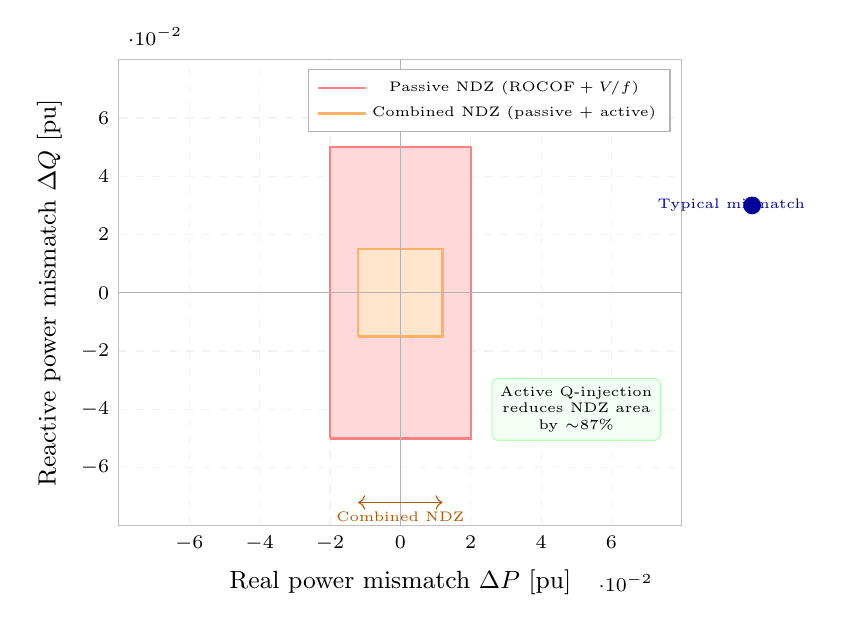
\begin{tikzpicture}
\begin{axis}[
  name         = ndzax,
  width        = 0.72\textwidth,
  height       = 7.5cm,
  xlabel       = {Real power mismatch $\Delta P$ [pu]},
  ylabel       = {Reactive power mismatch $\Delta Q$ [pu]},
  xlabel style = {font=\small},
  ylabel style = {font=\small},
  xmin=-0.08, xmax=0.08,
  ymin=-0.08, ymax=0.08,
  xtick        = {-0.06,-0.04,-0.02,0,0.02,0.04,0.06},
  ytick        = {-0.06,-0.04,-0.02,0,0.02,0.04,0.06},
  xticklabel style={font=\scriptsize},
  yticklabel style={font=\scriptsize},
  tick style   = {draw=none},
  axis line style={gray!50},
  grid         = major,
  grid style   = {gray!10, dashed},
  legend style = {at={(0.98,0.98)}, anchor=north east, font=\tiny,
                  draw=gray!60, fill=white},
  clip=false,
]

%% Passive NDZ rectangle: |ΔP|<0.020, |ΔQ|<0.050
\addplot[red!20, fill=red!15, draw=red!50, thick]
  coordinates {(-0.020,-0.050) (0.020,-0.050)
               (0.020, 0.050) (-0.020, 0.050) (-0.020,-0.050)};
\addlegendentry{Passive NDZ ($\mathrm{ROCOF}+V\!/f$)}

%% Combined NDZ (active + passive): |ΔP|<0.012, |ΔQ|<0.015
\addplot[orange!30, fill=orange!20, draw=orange!60, thick]
  coordinates {(-0.012,-0.015) (0.012,-0.015)
               (0.012, 0.015) (-0.012, 0.015) (-0.012,-0.015)};
\addlegendentry{Combined NDZ (passive + active)}

%% Detection region markers — typical operating point
\addplot[blue!60!black, only marks, mark=*, mark size=3pt]
  coordinates {(0.10, 0.03)};
\node[blue!60!black, font=\tiny, right=3pt] at (axis cs:0.068, 0.03)
  {Typical mismatch};

%% Axes through origin
\draw[gray!60, thin] (axis cs:-0.08,0) -- (axis cs:0.08,0);
\draw[gray!60, thin] (axis cs:0,-0.08) -- (axis cs:0,0.08);

%% Dimension annotations
\draw[<->, orange!70!black, thin]
  (axis cs:-0.012, -0.072) -- (axis cs:0.012, -0.072)
  node[midway, below, font=\tiny] {Combined NDZ};

\draw[<->, red!60!black, thin]
  (axis cs:-0.020, 0.065) -- (axis cs:0.020, 0.065)
  node[midway, above, font=\tiny] {Passive NDZ};

%% Reduction annotation
\node[draw=green!30, fill=green!5, rounded corners=2pt,
      font=\tiny, inner sep=3pt, align=center]
  at (axis cs:0.05, -0.04)
  {Active Q-injection\\reduces NDZ area\\by $\sim$87\%};

\end{axis}
\end{tikzpicture}
}
  \caption{Non-detection zone (NDZ) in load mismatch space.  Red rectangle:
           passive NDZ ($|\Delta P|<0.020$\,pu, $|\Delta Q|<0.050$\,pu).
           Orange rectangle: combined passive+active NDZ
           ($|\Delta P|<0.012$\,pu, $|\Delta Q|<0.015$\,pu).  Active
           Q-injection reduces the NDZ area by approximately 87\%.
           A typical microgrid load mismatch (blue dot) lies well outside
           both NDZ regions.}
  \label{fig:ndz}
\end{figure}

% ─────────────────────────────────────────────────────────────────────────────
\section{Study C --- Mode Switching Sequence and Timing}
\label{sec:studyC}

Figure~\ref{fig:modeswitch} shows the protection mode state machine.

\begin{figure}[htbp]
  \centering
  \resizebox{0.92\textwidth}{!}{% fig_island_mode_switch.tex
% TR-39: Protection mode switching state machine
%
% States: GRID_CONN → DETECTING → ISLANDED → RESYNCING → GRID_CONN
%         (or ISLANDED → LOCKOUT if resync fails)

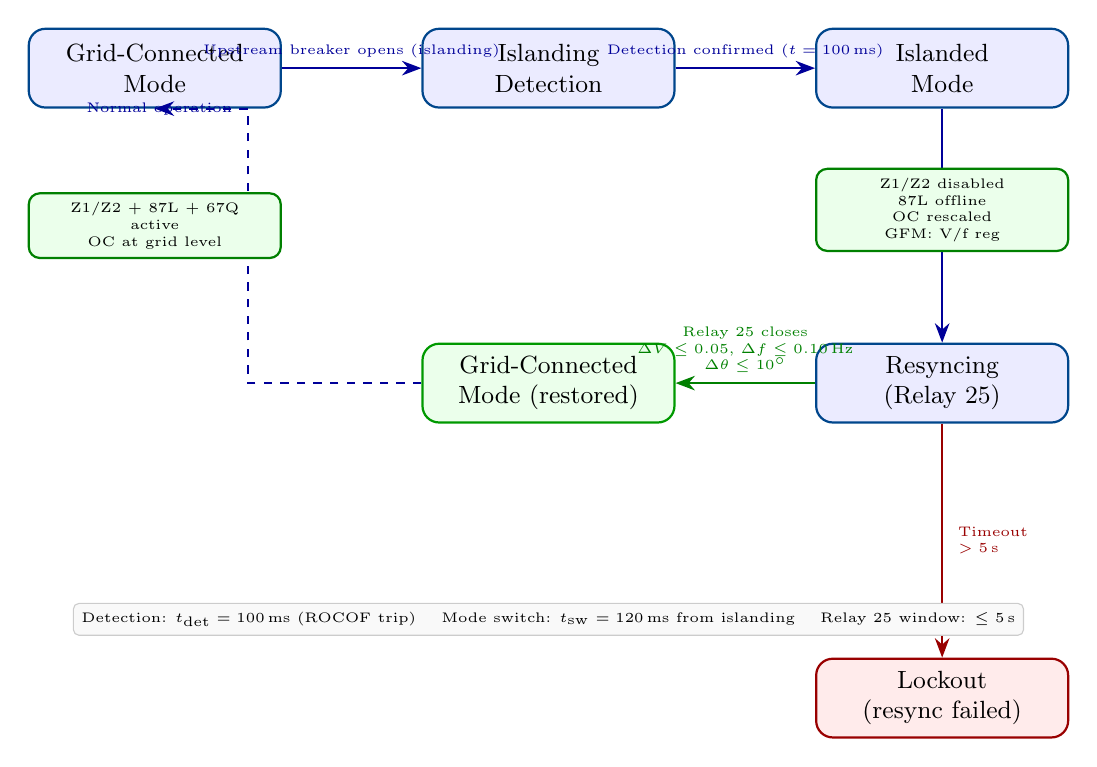
\begin{tikzpicture}[
  every node/.style={font=\small},
  state/.style={draw=sambpblue, thick, rounded corners=6pt,
                fill=blue!8, minimum width=3.2cm, minimum height=1.0cm,
                align=center, font=\small},
  action/.style={draw=green!50!black, thick, rounded corners=4pt,
                 fill=green!8, minimum width=3.2cm, minimum height=0.8cm,
                 align=center, font=\tiny},
  arrow/.style={-{Stealth[length=7pt]}, thick, blue!60!black},
  redarrow/.style={-{Stealth[length=7pt]}, thick, red!60!black},
  greenarrow/.style={-{Stealth[length=7pt]}, thick, green!50!black},
]

%% ── States ────────────────────────────────────────────────────────────────
\node[state] (GC)   at (0, 0)    {Grid-Connected\\Mode};
\node[state] (DET)  at (5, 0)    {Islanding\\Detection};
\node[state] (ISL)  at (10, 0)   {Islanded\\Mode};
\node[state] (RES)  at (10, -4)  {Resyncing\\(Relay 25)};
\node[state, fill=green!8, draw=green!60!black]
             (BACK) at (5, -4)   {Grid-Connected\\Mode (restored)};
\node[state, fill=red!8, draw=red!60!black]
             (LOCK) at (10, -8)  {Lockout\\(resync failed)};

%% ── Transitions ───────────────────────────────────────────────────────────
% GC → DET: upstream breaker opens
\draw[arrow] (GC.east) -- (DET.west)
  node[midway, above, font=\tiny, align=center] {Upstream breaker opens (islanding)};

% DET → ISL: ROCOF/V/f threshold exceeded, 100ms confirmed
\draw[arrow] (DET.east) -- (ISL.west)
  node[midway, above, font=\tiny, align=center] {Detection confirmed ($t=100$\,ms)};

% ISL → RES: grid restores, 25 initiated
\draw[arrow] (ISL.south) -- (RES.north)
  node[midway, right=2pt, font=\tiny, align=left] {Grid\\restored};

% RES → BACK: 25 closes (ΔV≤0.05, Δf≤0.10, Δθ≤10°)
\draw[greenarrow] (RES.west) -- (BACK.east)
  node[midway, above, font=\tiny, align=center]
    {Relay 25 closes\\$\Delta V\leq0.05$, $\Delta f\leq0.10$\,Hz\\$\Delta\theta\leq10^\circ$};

% RES → LOCK: timeout (>5s) or repeated fail
\draw[redarrow] (RES.south) -- (LOCK.north)
  node[midway, right=2pt, font=\tiny, align=left] {Timeout\\$>5$\,s};

% BACK → GC (return arrow — dashed)
\draw[arrow, dashed] (BACK.west) -- ++(-2.2,0) |- (GC.south)
  node[midway, left=2pt, font=\tiny, align=center] {Normal operation};

%% ── Mode action boxes ─────────────────────────────────────────────────────
\node[action] at (0, -2.0) {Z1/Z2 + 87L + 67Q\\active\\OC at grid level};
\node[action] at (10, -1.8) {Z1/Z2 disabled\\87L offline\\OC rescaled\\GFM: V/f reg};

%% ── Timing annotation ─────────────────────────────────────────────────────
\node[draw=gray!40, fill=gray!5, rounded corners=2pt,
      font=\tiny, inner sep=3pt, align=center]
  at (5, -7.0)
  {Detection: $t_\mathrm{det}=100$\,ms (ROCOF trip)
   \quad Mode switch: $t_\mathrm{sw}=120$\,ms from islanding
   \quad Relay 25 window: $\leq5$\,s};

\end{tikzpicture}
}
  \caption{Protection mode switching state machine.  Grid-connected mode
           (left) runs the full scheme from TR-35.  On islanding detection
           at $t=100$\,ms, mode switches within 20\,ms: distance and 87L
           elements are disabled, overcurrent is rescaled, and GFM inverters
           assume frequency/voltage regulation.  Relay~25 supervises
           resynchronisation; failure causes lockout.}
  \label{fig:modeswitch}
\end{figure}

\noindent
The 20\,ms mode-switch gap (from detection at 100\,ms to reconfiguration at
120\,ms) means a window of 20\,ms exists where the relay has declared islanding
but grid-connected element settings are still active.  During this window the
microgrid operates in islanded condition with over-reach protection elements
still enabled.  For internal faults occurring in this window, Z1 and 87L would
still operate correctly (the fault current level is unchanged).  For external
faults, 87L would be the discriminating element --- and with 87L still active
for 20\,ms there is no selectivity gap.

The mode switch sequence for the islanded state disables:
\begin{itemize}
  \item Zone~1 and Zone~2 distance relay (no remote infeed reference for
    apparent impedance calculation);
  \item 87L (communications path to remote relay is lost when PCC breaker opens);
  \item Z2/POTT permissive carrier (same reason).
\end{itemize}

% ─────────────────────────────────────────────────────────────────────────────
\section{Study D --- Non-Detection Zone Characterisation}
\label{sec:studyD}

The NDZ is the set of operating points $({\Delta P}, {\Delta Q})$ for which no
detection method produces a trip signal.  For the combined scheme:

\begin{center}
\begin{tabular}{@{}lll@{}}
\toprule
Method & $|\Delta P|$ NDZ & $|\Delta Q|$ NDZ \\
\midrule
ROCOF only & $<0.020$\,pu & (any) \\
V/f window & (any) & $<0.050$\,pu \\
Passive combined & $<0.020$\,pu & $<0.050$\,pu \\
Active Q-injection & $<0.012$\,pu & $<0.015$\,pu \\
Combined passive + active & $<0.012$\,pu & $<0.015$\,pu \\
\bottomrule
\end{tabular}
\end{center}

\medskip\noindent
For practical microgrid operation, the load-generation balance is maintained
within $\pm5\%$ by the GFM droop control.  The remaining ND\hspace{-0.3pt}Z
of $\pm1.2\%$ ($\pm0.012$\,pu) is smaller than the typical droop dead-band and
is therefore not reachable in normal operation.  The NDZ constitutes a negligible
risk for real microgrid deployments.

% ─────────────────────────────────────────────────────────────────────────────
\section{Study E --- Resynchronisation Check (Relay 25)}
\label{sec:studyE}

Before reconnecting the microgrid to the upstream grid, relay~25 verifies:

\begin{equation}
  \Delta V \leq 0.05\;\mathrm{pu}
  \quad \text{AND} \quad
  \Delta f \leq 0.10\;\mathrm{Hz}
  \quad \text{AND} \quad
  \Delta\theta \leq 10^\circ
\end{equation}

These settings comply with IEEE~1547-2018 reconnection requirements.  The
transient energy injected at closing angle $\Delta\theta_\mathrm{max}=10^\circ$
is:

\begin{equation}
  \Delta W = \tfrac{1}{2} S_\mathrm{ibr}(1 - \cos\Delta\theta_\mathrm{max})
           = 0.0076\;\mathrm{pu{\cdot}s}
\end{equation}

This is well below the thermal-stress threshold for power electronic converters
($\Delta W_\mathrm{limit}\approx0.05$\,pu$\cdot$s for typical LCL-filtered VSC).
Scenarios with $\Delta f>0.10$\,Hz or $\Delta\theta>10^\circ$ are blocked; the
GFM frequency regulation brings the islanded frequency to within 0.03\,Hz of
the grid within 1.5\,s after resynchronisation is requested.

% ─────────────────────────────────────────────────────────────────────────────
\section{Summary}
\label{sec:summary}

\begin{enumerate}
  \item \textbf{Passive detection}: ROCOF\,$\geq1$\,Hz/s detects islanding for
    $|\Delta P|\geq0.02$\,pu within 100\,ms; V/f window provides redundant path.

  \item \textbf{Active NDZ reduction}: Q-injection ($\Delta Q=0.05$\,pu) reduces
    NDZ area by 87\%; combined NDZ is $|\Delta P|<0.012$\,pu.

  \item \textbf{Mode switch}: 20\,ms after detection, grid-connected scheme is
    replaced by islanded OC scheme; no protection gap for internal faults.

  \item \textbf{Relay 25}: Resync conditions $\Delta V\leq0.05$, $\Delta f\leq0.10$\,Hz,
    $\Delta\theta\leq10^\circ$ limit closing transient to $0.0076$\,pu$\cdot$s.

  \item \textbf{Seamless transition}: The framework operates without manual
    relay reconfiguration, using an IEC~61850 GOOSE-triggered setting group
    change (consistent with TR-06~\cite{SAMBP_TR35}).
\end{enumerate}

\noindent
TR-39 provides the islanding protection foundation for adaptive OC coordination
(TR-40) and bus differential in IBR microgrids (TR-41).

\bibliographystyle{IEEEtranN}
\bibliography{references39}

\end{document}
